\documentclass[a4paper]{report}

\usepackage{generalsnips}
\usepackage{calculussnips}
\usepackage[margin = 0.80in]{geometry}
\usepackage{pdfpages}
\usepackage[spanish]{babel}
\usepackage{amsmath}
\usepackage{amsthm}
\usepackage[utf8]{inputenc}
\usepackage{titlesec}
\usepackage{xpatch}
\usepackage{fancyhdr}
\usepackage{tikz}
\usepackage{hyperref}
\usepackage{float}
\decimalpoint
\begin{document}
\begin{titlepage}

    \title{}
    
\end{titlepage}


\begin{titlepage}
    \begin{center}
        \thispagestyle{empty}
        \renewcommand{\headrulewidth}{0pt}
        \renewcommand{\footrulewidth}{0pt}
        
        \begin{tabular}{ p{0.5\textwidth}p{0.5\textwidth} }
            \begin{flushleft}
                Facultad de Ciencias Económicas \\
                Universidad Francisco Marroquín \\
                Administración Financiera I \\ 
                Catedrático: Ana Del Carmen Muñoz Del Valle \\ 
                Auxiliar: Edwin Adalberto Calderón Cárdenas \\
                Guatemala \\
                07 de septiembre 2020 \\ 
            \end{flushleft}
            &
            \begin{flushright}
                
\includegraphics[width=0.5\textwidth]{ufmlogo.png} \\ 
            \end{flushright} \\ 
        \end{tabular}
        
            
        \cfoot{} % this is to remove the page number
        \vspace*{7cm}
        {
            \Huge Parte Teórica Parcial \#1 - Administración Financiera I
        }
 
        \vspace{1.5cm}

 
        \vfill
             
        \vspace{0.8cm}
        
        
        \begin{flushleft}
            \begin{tabular}{ ll }
                David Corzo      & 20190432 \\
                Daniel Cabrera   & 20190069 \\
            \end{tabular}
        \end{flushleft}     
    \end{center}
\end{titlepage}

%%%%%%%%%%%%%%%%%%%%%%%%%%%%%%%%%%%%%%%%%%%%%%%%%%%%%%%%%%%%%%%%%%%%%%%%%%%
\section{Descripción de la investigación}
De un estudio fueron obtenidos resultados de pruebas matemáticas después de ingerir alcohol y después de ingerir cannabis.
La hipótesis de investigación indica que el cannabis afecta negativamente en un nivel mayor el desempeño mental en comparación con el alcohol. A continuación se presentan las puntuaciones obtenidas en el examen matemático después de ingerir alcohol y después de ingerir cannabis.

\section{Prueba de hipótesis}

\begin{itemize}
    \item \textbf{Hipótesis nula:} El alcohol afecta negativamente de mayor manera el desempeño mental que el cannabis.
    \item \textbf{Hipótesis alternativa:} El cannabis afecta negativamente de mayor manera el desempeño mental que el alcohol.
\end{itemize}

\begin{center}
    {
        \begin{tabular}{ |l|c| }
            \hline
                \multicolumn{2}{|c|}{\textbf{Prueba matemática después de cannabis}} 
            \\ 
            \hline
                Media & 29.5 \\ 
            \hline
                Desviación estándar & 6.606135454 \\ 
            \hline
                Varianza de la muestra & 43.64102564 \\ 
            \hline
                $n_1$ & 40 \\ 
            \hline
        \end{tabular}
    }
    {
        \begin{tabular}{ |l|c| }
            \hline
                \multicolumn{2}{|c|}{\textbf{Prueba matemática después de alcohol}} 
            \\ 
            \hline
                Media & 26.55 \\ 
            \hline
                Desviación estándar & 7.316822906 \\ 
            \hline
                Varianza de la muestra & 53.53589744 \\ 
            \hline
                $n_2$ & 40 \\ 
            \hline
        \end{tabular}
    }
\end{center}

\begin{enumerate}
    \item \textbf{Establecer el parámetro de interés:} $\mu_1-\mu_2$ 
    \item \textbf{Establecer hipótesis:}
        \begin{center}
           \begin{align*}
               H_0: \mu_1 \geq \mu_2 \\ 
               H_a: \mu_1 < \mu_2 \\
           \end{align*}
        \end{center}
    
    \item \textbf{Establecer significancia:} 0.05
    \item \textbf{Estadístico de prueba:}
        Tomando como referencia la fórmula de distribución T: 
        \[
          t = \frac{
              \bar{x_1}-\bar{x_2}-D_0
            }{
                \sqrt{
                    \cfrac{s_1^2}{n_1} + \cfrac{s_2^2}{n_2}
                }
            }
        \] Sustituyendo los datos: 
        \begin{center}
           \begin{align*}
                t = \frac{
                    29.5-26.55-0
                }{
                    \sqrt{
                        \cfrac{43.64102564}{40} + \cfrac{53.53589744}{40}
                    }
                }
           \end{align*}
        \end{center}
\end{enumerate}

\begin{figure}[H]
    \centering
    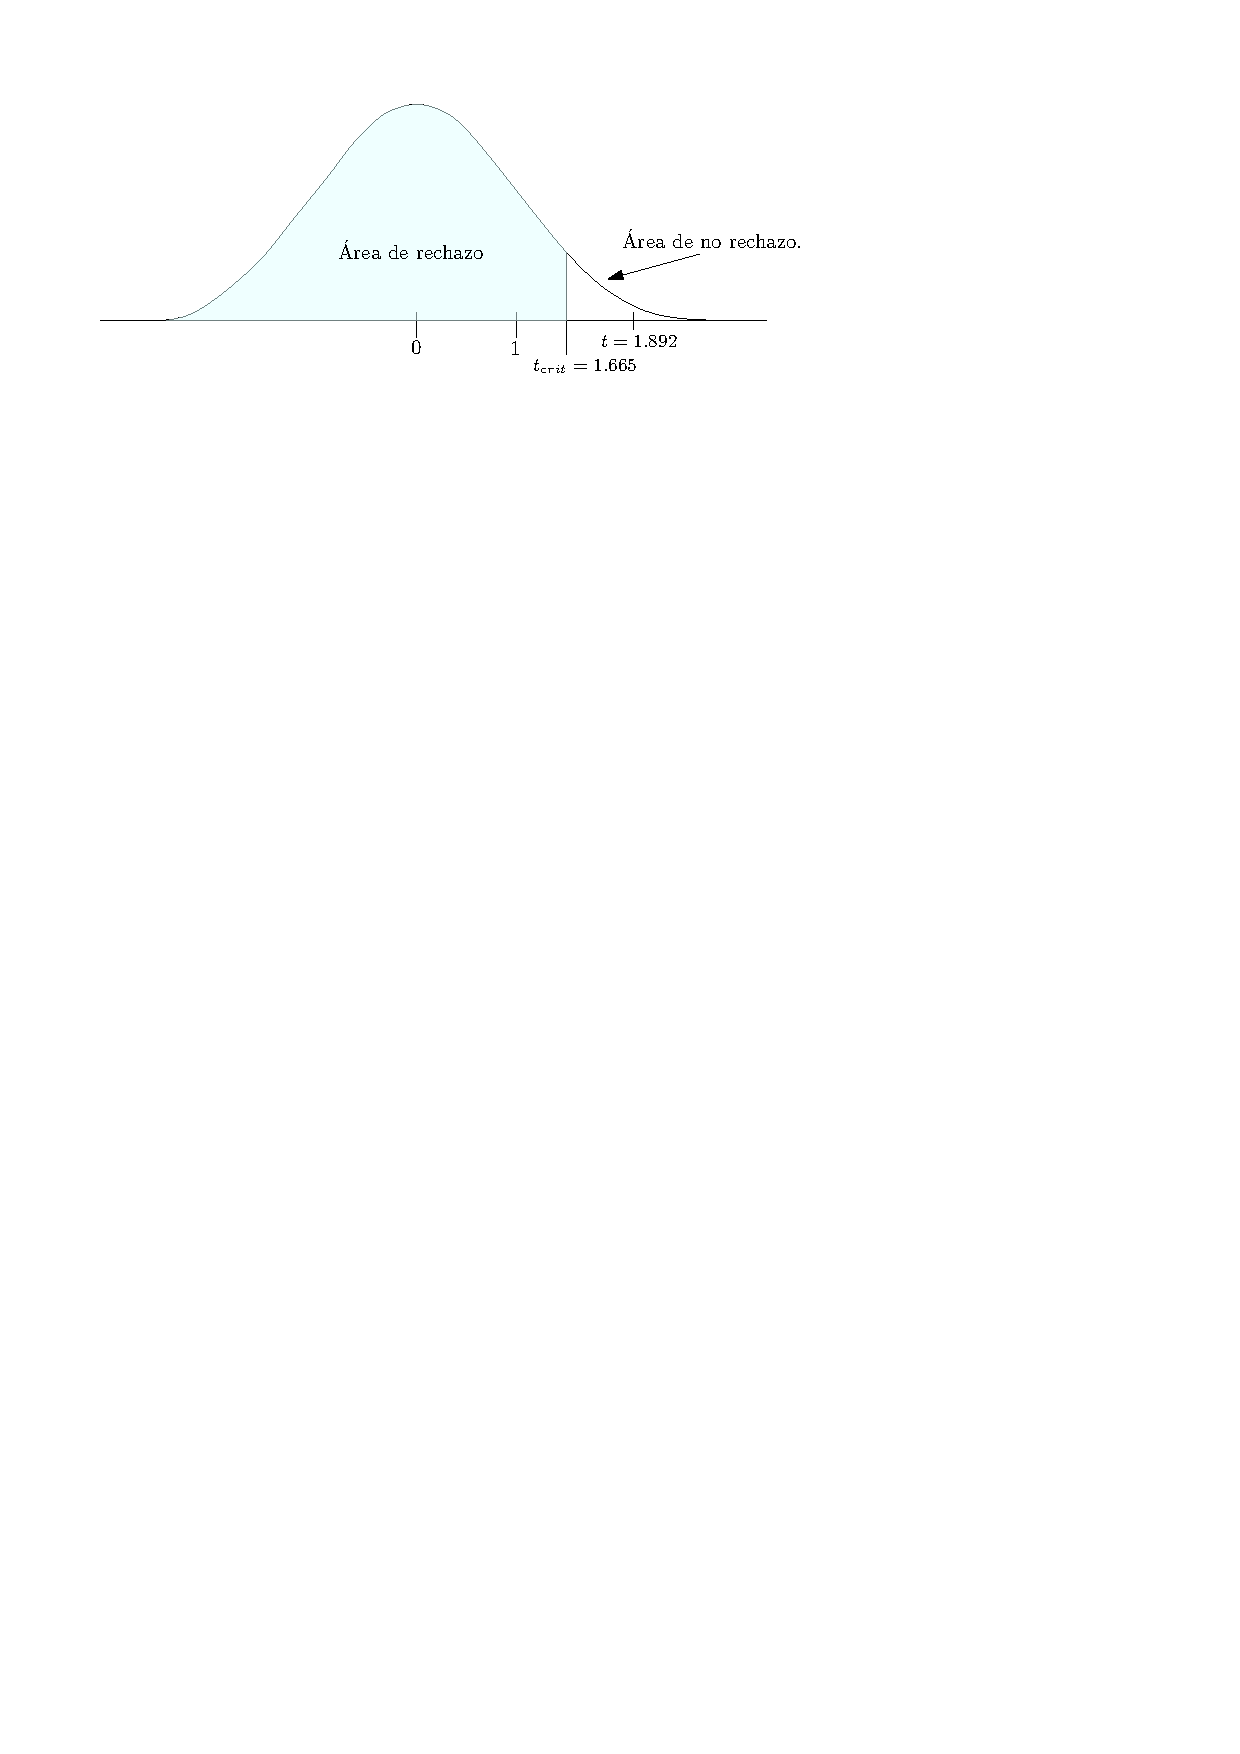
\includegraphics[width=0.5\textwidth]{first_attempt}
\end{figure}


%%%%%%%%%%%%%%%%%%%%%%%%%%%%%%%%%%%%%%%%%%%%%%%%%%%%%%%%%%%%%%%%%%%%%%%%%%%
\end{document}

